\chapter{Modely}

V~sekcii \ref{sec:hmm-alignment} sme si zadefinovali HMM pre zarovnávanie sekvencií (obr. \ref{fig:simple-model}).
V~našom riešení sme predstavili 2 modifikácie pôvodného HMM na zakomponovanie dodatočnej informácie, pričom sme využili klasifikátory. V~oboch modeloch sú klasifikátory rovnaké, aj s~rovnakým postupom trénovania. Líši sa len trénovanie samotného HMM a architektúra modelu.

\section{Model s~klasifikátorom ako emisiou}

V~tomto modeli sme nahradili emisné tabuľky stavov výstupom z~klasifikátora.
Model teda bude vyzerať rovnako, aj pravdepodobnosti prechodov zostanú, ale emisná pravdepodobnosť sa nahradí výstupom z~klasifikátora.

\begin{figure}[htp]
    \centering
    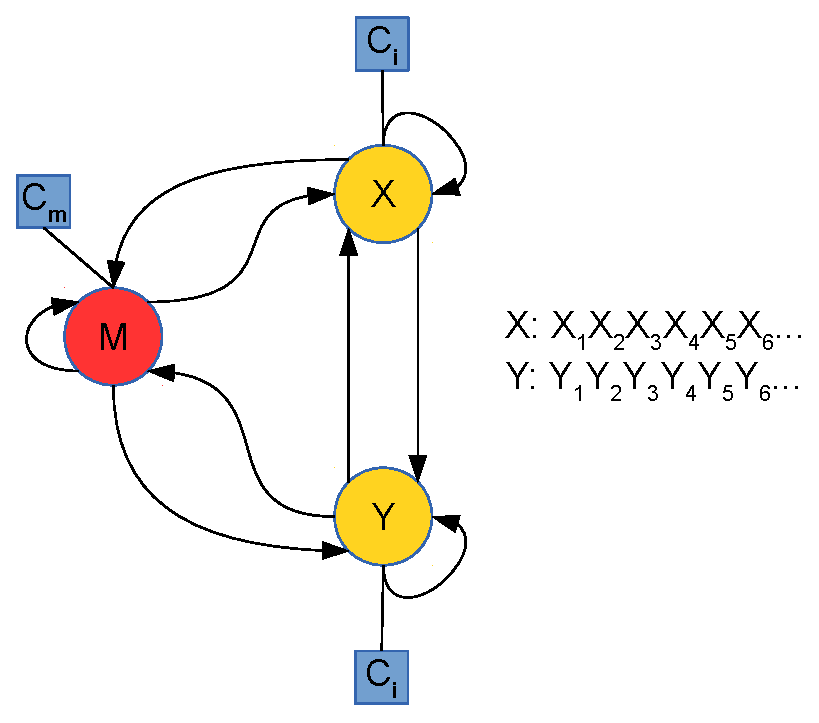
\includegraphics[width=.5\textwidth]{images/model_clf}
    \caption{Model s~klasifikátorom ako emisiou}
\end{figure}


Problémom tohto modelu je, že výstup klasifikátora nezodpovedá emisným pravdepodobnostiam, ale akejsi istote klasifikátora o~tom, že dve pozície majú byť zarovnané k~sebe. Hodnoty z~klasifikátora teda nesumujú do 1 a model nie je celkom korektný. V~praxi sa však ukázalo, že to až tak nevadí, avšak o~takomto modeli už nemôžme hovoriť ako o~pravdepodobnostnom. Je len inšpirovaný HMM.

V~tomto modeli sme trénovali iba tranzície, emisie sme mali priamo z~natrénovaného klasifikátora.

\section{Model s~klasifikátorovou páskou}
(\todo alebo s orákulom?)

Na to aby sme vyriešili problém s~korektnosťou predošlého modelu, navrhli sme alternatívny model, ktorý je korektný pravdepodobnostný model, ktorý navyše modeluje aj výstup z~klasifikátora.
Nemodelujeme teda len dvojicu sekvencií, ale aj sekvenciu výstupov klasifikátora vo forme pásky.
Pásku s~výstupom z~klasifikátora vieme považovať za akúsi pomôcku pre náš zarovnávač.

\begin{figure}[htp]
    \centering
    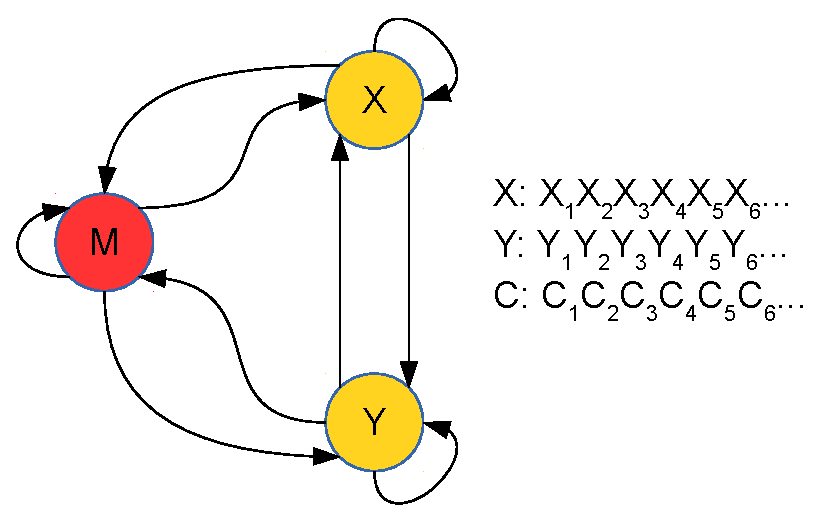
\includegraphics[width=.5\textwidth]{images/model_clf_paska}
    \caption{Model s~klasifikátorovou páskou}
\end{figure}

Keďže stále ide o párový HMM, pásku si musíme predstaviť ako cestu v 2D tabuľke výstupov klasifikátorov, ktorá sa zhoduje s cestou zarovnania. Teda ak sa pohneme horizontálne  alebo vertikálne, používame Indel klasifikátor a ak sa pohneme diagonálne tak použijeme Match klasifikátor.

\subsection{Trénovanie modelu} % (fold)
Pri tomto modeli stojí za zmienku aj spôsob trénovania.
Trénovali aj tranzície aj emisie, pričom základný princíp ostáva taký, ako sme si ho popísali v~sekcii \ref{subsec:hmmtraining}.
Zaujímavé je trénovanie emisií klasifikátora. Z~dôvodu lepšej vizualizácie a ďalších dôvodov, ktoré uvedieme neskôr sa nám hodí modelovať pravdepodobnosti $P(C|X \cap Y)$. Ukážeme si, že pravdepodobnosť $P(X \cap Y \cap C)$ vieme rozložiť pomocou $P(C|X \cap Y)$.

V~Match stave modelujeme 3 náhodné premenné -- $X$, $Y$ a $C$, pričom tieto náhodné premenné sú nezávislé. Teda platí $P(X \cap Y \cap C) = P(X \cap Y)P(C)$.
$P(X \cap Y)$ poznáme z~frekvenčnej tabuľky a $P(C)$ vieme rozložiť pomocou nasledujúcej vety.

\begin{vt}[Veta o~úplnej pravdepodobnosti]
Nech $A_1\dots A_n$ tvoria rozklad univerza~$\Omega$ a nech $B$ je udalosť, potom
$$P(B) = \sum_{i=1}^n P(B|A_i)P(A_i)$$
\end{vt}

Máme teda
$$P\left[C=c\right] = \sum_{\forall x\in X, y \in Y} P\left[C=c | X=x \wedge Y=y\right] P\left[X=x \wedge Y=y\right],$$
pričom druhý člen poznáme a $P\left[C=c | X=x \wedge Y=y\right]$ už vieme ľahko dopočítať. Keď máme fixnuté dve bázy, vieme vybrať z~trénovacej sekvencie všetky pozície, kde sú zarovnané tieto bázy a vypočítať distribúciu C.

Pre Indel stav postupujeme analogicky, ibaže namiesto $P(X \cap Y)$ máme buď $P(X)$ alebo $P(Y)$ podľa toho, ktorý stav práve počítame.

Vieme teda pravdepodobnosť emisie $(x, y, c)$ Match stave vypočítať ako $$P\left[C=c \wedge X=x \wedge Y=y\right] = P\left[C=c | X=x \wedge Y=y\right] P\left[X=x \wedge Y=y\right]$$ a pravdepodobnosť emisie $(x, c)$ resp. $(y, c)$  v~Inzert stavoch pomocou
\begin{align*}
P\left[C=c \wedge X=x\right] &= P\left[C=c | X=x\right] P\left[X=x\right]\\
P\left[C=c \wedge Y=y\right] &= P\left[C=c | Y=y\right] P\left[Y=y\right].
\end{align*}

Klasifikátor môže ľubovoľnú vrátiť hodnotu z intervalu $\left<0,1 \right>$. Doteraz používané HMM boli diskrétne, čiže nepracovali so spojitými výstupmi. Môžme buď hodnoty diskretizovať, alebo použiť spojité HMM definované napr. v \cite{huang1989multiple}. Diskretizovať hodnoty môžme 2 spôsobmi, buď priamo -- spočítať histogram pre trénovacie dáta, alebo nepriamo -- interpolovať vstupnú vzorku na celý interval, napr. pomocou zmesi gausovských rozdelení a potom toto rozdelenie diskretizovať. Druhá spomenutá metóda má výhodu v tom, že vyhladí šum, ale treba s ňou narábať opatrne, aby sme nezaviedli príliš veľkú nepresnosť.

\todo spojité hmm

Ak použijeme spojitý HMM, tak využijeme interpoláciu pomocou zmesi gausovských rozdelení a to budeme brať ako hustotu výstupu klasifikátora.

\todo obrázok toho čo ideme robiť

% Klasifikátorovú pásku sme generovali pomocou oboch klasifikátorov, pričom v~Match stave sme použili Match klasifikátor a v~Insert stavoch Indel klasifikátor.
% Výstupy z~klasifikátora sme rozdelili do 10 košov rovnomerne na intervale <0, 1>.

% subsection Trénovanie modelu (end)
